\documentclass[11pt,a4paper]{article}

\usepackage{url,,}
\usepackage{graphicx}
\usepackage{hyperref}
\usepackage{amsfonts}
\usepackage{amssymb}
\usepackage{amsmath}
\usepackage{amsfonts}
\usepackage{amssymb}
\usepackage{amsmath}
\usepackage{multirow}
\usepackage{listings}
\usepackage{fullpage}
\usepackage{fancyhdr,a4wide}
\usepackage{makeidx}
\usepackage{placeins}
\usepackage[procnames,noindent]{lgrind}

\lstset{ %
language=VHDL,                % choose the language of the code
basicstyle=\footnotesize,       % the size of the fonts that are used for the code
showstringspaces=false,         % underline spaces within strings
%numbers=left,                   % where to put the line-numbers
%numberstyle=\footnotesize,      % the size of the fonts that are used for the line-numbers
%stepnumber=1,                   % the step between two line-numbers. If it's 1 each line will be numbered
%numbersep=5pt,                  % how far the line-numbers are from the code
%backgroundcolor=\color{white},  % choose the background color. You must add \usepackage{color}
showspaces=false,               % show spaces within strings adding particular underscores
showtabs=false,                 % show tabs within strings adding particular underscores
escapeinside={\%*}{*)}          % if you want to add a comment within your code
}

\begin{document}	

\begin{titlepage}

\thispagestyle{fancy}
\lhead{}
\chead{
\large{\textit{
Informatics and Mathematical Modelling\\
Technical University of Denmark}}}
\rhead{}
\rule{0pt}{50pt}
\vspace{3cm}

\begin{center}

 	\huge{\textbf{02207 : Advanced Digital Design Techniques}}\\
 	\vspace{1cm}
 	\huge{Exercise of Retiming}\\
 	\vspace{1cm}
 	\huge{\textit{LAB 3}}\\
 	\vspace{1cm}
 	\huge{Group \textit{dt07}}\\
\end{center}

\vspace{4cm}

\begin{flushright}
	\LARGE{Markku Eerola (s053739)}\\
	\vspace{0.3cm}
	\LARGE{Rajesh Bachani (s061332)}\\
	\vspace{0.3cm}
	\LARGE{Josep Renard (s071158)}\\
\end{flushright}
\cfoot{\today}
\end{titlepage}

%\begin{abstract}
%\centering
%Abstract to be created.
%\end{abstract}

%-----------------------------------------------------------
\newpage 
\tableofcontents

\newpage 
\section{Introduction}
This document is report of the third exercise on DTU course Advanced Digital Design. In this exercise we studied the concept of retiming using digit recurrence division implementation with radix-4 and carry-save adder.

In the introductory section we will briefly explain the concept of retiming, the original circuit and the retimed circuit. In the next section we will explain how the retimed circuit was implemented ie. what changes we made to the original circuit. In the last two sections we will present the power reports and cell counts of the two designs and discuss the results.

\subsection{Retiming}
% to just explain what retiming is - the concept and its purpose. that we need to retime circuits manually - so that the synthesizer could identify two different paths easily and perform low power synthesis for the non critical path.
Retiming is an optimizing technique where structural location of registers is manually moved without affecting the functionality of the circuit in order to improve its performance. In our case the motivation was to create slack on a non-critical path, and to have the synthesizer substitute HS cells with LL cells on this path thus lowering the power dissipation in the whole circuit. According to the lecture slides the circuit we were studying should gain approximately 30\% power savings from retiming.

\subsection{Simple Design for Division}
%explain briefly the circuit for division. mention about the critical path in the circuit.
The original design upon which we aimed to improve with the retiming is presented in figure 1.

\begin{figure}
	\centering
		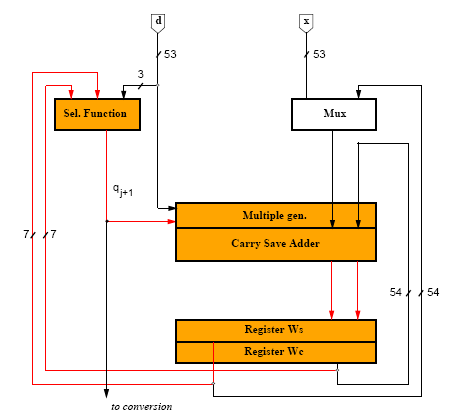
\includegraphics{./noretiming.PNG}
	\caption{Figure 1: Digit recurrence division}
	\label{fig:noretiming}
\end{figure}

The Sel. function -block implements the quotient digit selection function. The selection function determines a 4-bit quotient digit using 3 most significant bits of the divisor d and 7 most significant bits from the results stored in registers Ws and Wc.

The MUX block selects the input for the divisor multiplication between the dividend, which is used only in the initialization phase of the division algorithm, and the result of the substraction of the quotient digit/divisor multiplication result from the dividend. The substraction result is stored in register Ws.

The Multiple gen. -block implements the divisor multiplication ie. it multiplies the divisor d with the 4-bit quotient digit.

The Carry Save Adder -block implements the substraction of the result of the divisor multiplication from the dividend. The substraction is done with a carry-save adder as the name of the block suggests.

The registers Ws and Wc store the carry and the sum from the carry-save adder respectively.

The critical path of this circuit is marked with red arrows in the figure.

\subsection{Design for Division using Retiming}
%explain in detail the circuit for division using retiming. we should argue what is expected from this, and how we should be able to save power in this.
The retimed design is presented in figure 2.

\begin{figure}
	\centering
		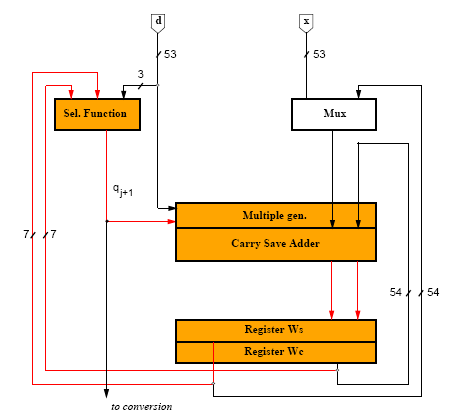
\includegraphics{./noretiming.PNG}
	\caption{Figure 1: Digit recurrence division retimed}
	\label{fig:retiming}
\end{figure}



\subsection{Authors by Section}
\begin{itemize}
\item \textit{Rajesh Bachani} 
\item \textit{Josep Renard} 
\item \textit{Markku Eerola} 
\end{itemize}

\section{Implementation of Division using Retiming}
\label{section:impl}
%explain specifically the changes that were implemented for using the retimed circuit for division. this could also include parts of the VHDL, but mostly it should concentrate on highlighting the changes in terms of the connections between the components.
%we would not have any section for implementation, giving the code, since there is a lot of code in the whole thing. so we should try and just explain all the changes in the code here only.
\section{Power Report and Cell Count}
\label{section:power}
% put the reports from the power analysis of both the designs here. also, give a short recap kind of a table here. also, write about the cells here.
\section{Discussion}
\label{section:discussion}
%discuss the report at length here. we should clearly justify the results, by explaining why the SVT cells count has reduced and HVT has increased, and why the cell internal power has reduced. ofcourse this was expected, but nice explanation is needed here. 
\end{document}